\PassOptionsToPackage{unicode=true}{hyperref} % options for packages loaded elsewhere
\PassOptionsToPackage{hyphens}{url}
%
\errorcontextlines 10000
\documentclass[]{tufte-handout}
\usepackage{lmodern}
\usepackage{amssymb,amsmath}
\usepackage{ifxetex,ifluatex}
\usepackage{fixltx2e} % provides \textsubscript
\ifnum 0\ifxetex 1\fi\ifluatex 1\fi=0 % if pdftex
  \usepackage[T1]{fontenc}
  \usepackage[utf8]{inputenc}
  \usepackage{textcomp} % provides euro and other symbols
\else % if luatex or xelatex
  \usepackage{unicode-math}
  \defaultfontfeatures{Ligatures=TeX,Scale=MatchLowercase}
\fi
% use upquote if available, for straight quotes in verbatim environments
\IfFileExists{upquote.sty}{\usepackage{upquote}}{}
% use microtype if available
\IfFileExists{microtype.sty}{%
\usepackage[]{microtype}
\UseMicrotypeSet[protrusion]{basicmath} % disable protrusion for tt fonts
}{}
\IfFileExists{parskip.sty}{%
\usepackage{parskip}
}{% else
\setlength{\parindent}{0pt}
\setlength{\parskip}{6pt plus 2pt minus 1pt}
}
\usepackage{fancyvrb}
\usepackage{hyperref}
\hypersetup{
            pdftitle={Fondements de programmation},
            pdfauthor={Hugo Leblanc},
            pdfborder={0 0 0},
            breaklinks=true}
\urlstyle{same}  % don't use monospace font for urls
%\VerbatimFootnotes % allows verbatim text in footnotes
\usepackage{listings}
\newcommand{\passthrough}[1]{#1}
\usepackage{graphicx,grffile}
\makeatletter
\def\maxwidth{\ifdim\Gin@nat@width>\linewidth\linewidth\else\Gin@nat@width\fi}
\def\maxheight{\ifdim\Gin@nat@height>\textheight\textheight\else\Gin@nat@height\fi}
\makeatother
% Scale images if necessary, so that they will not overflow the page
% margins by default, and it is still possible to overwrite the defaults
% using explicit options in \includegraphics[width, height, ...]{}
\setkeys{Gin}{width=\maxwidth,height=\maxheight,keepaspectratio}
\setlength{\emergencystretch}{3em}  % prevent overfull lines
\providecommand{\tightlist}{%
  \setlength{\itemsep}{0pt}\setlength{\parskip}{0pt}}
\setcounter{secnumdepth}{0}
% Redefines (sub)paragraphs to behave more like sections
\ifx\paragraph\undefined\else
\let\oldparagraph\paragraph
\renewcommand{\paragraph}[1]{\oldparagraph{#1}\mbox{}}
\fi
\ifx\subparagraph\undefined\else
\let\oldsubparagraph\subparagraph
\renewcommand{\subparagraph}[1]{\oldsubparagraph{#1}\mbox{}}
\fi

% set default figure placement to htbp
\makeatletter
\def\fps@figure{htbp}
\makeatother

\usepackage{xcolor}

\definecolor{mLightGreen}{HTML}{14B03D}


\usepackage[framed]{matlab-prettifier}
\lstset{frame=single,numbers=left}
\hypersetup{colorlinks=true,urlcolor=blue}

\title{Fondements de programmation}
\author{Hugo Leblanc}
\date{Cours 1}

\renewcommand\allcapsspacing[1]{{\addfontfeature{LetterSpace=15}#1}}
\renewcommand\smallcapsspacing[1]{{\addfontfeature{LetterSpace=10}#1}}

\begin{document}
\maketitle

\hypertarget{environnement}{%
\section{Environnement}\label{environnement}}

\hypertarget{current-folder}{%
\subsection{Current Folder}\label{current-folder}}

Le dossier courant\footnote{\href{https://www.mathworks.com/help/matlab/learn_matlab/desktop.html}{Desktop
  Basics}} représente l'espace de travail utilisé pour l'utilisation de
scripts ou fonctions. Pour pouvoir utiliser les programmes que nous
allons créer, il faut que ceux-ci soient dans le dossier courant. On
peut modifier le dossier courant avec la barre d'exploration au-dessus
de la fenêtre.

\hypertarget{command-window}{%
\subsection{Command Window}\label{command-window}}

La fenêtre de commande est l'interface principale dans MATLAB. Elle
permet de recevoir les instructions\footnote{\href{https://www.mathworks.com/help/matlab/matlab_env/enter-statements-in-command-window.html}{Enter
  Statements in Command Window}} qui seront ensuite exécutées.

\hypertarget{workspace}{%
\subsection{Workspace}\label{workspace}}

L'espace de travail représente la mémoire de MATLAB. C'est la
représentation des différentes variables qui sont disponibles pour
l'exécution.

\hypertarget{editor}{%
\subsection{Editor}\label{editor}}

L'éditeur est l'endroit où nous travaillerons le plus. C'est ici que
nous pouvons écrire nos scripts et fonctions qui seront la base de nos
programmes. Il est à mentionner que l'éditeur utilise une barre d'outils
avec plusieurs fonctionnalités propres à l'éditeur.

\hypertarget{concepts-fondamentaux-de-matlab}{%
\section{Concepts fondamentaux de
MATLAB}\label{concepts-fondamentaux-de-matlab}}

\hypertarget{instructions}{%
\subsection{Instructions}\label{instructions}}

Une instruction\footnote{``command'' ou ``statement'' en anglais.} est
l'élément de base que MATLAB traite dans un programme. Une instruction
peut exécuter une expression mathématique, appeler une fonction
spécifique ou prendre des décisions par rapport à un état ou une
condition. Un programme est constitué d'une multitude d'instructions qui
sont exécutées à la chaine par MATLAB. MATLAB est seulement capable
d'exécuter une instruction à la fois et doit attendre de compléter
l'instruction courante avant de pouvoir en exécuter une autre. Deux
méthodes de bases nous permettent d'utiliser des instructions: La
première et la plus directe est d'utiliser la fenêtre de commande ou
``Command Window''\footnote{L'invite de commande est représentée par
  deux signes plus grand que (\passthrough{\lstinline!>>!}). Cela
  indique que MATLAB est prêt à recevoir une nouvelle instruction.}.
Pour exécuter une instruction, on écrit l'instruction après l'invite de
commande suivit de la touche \passthrough{\lstinline!Entrer!} pour
exécuter l'instruction. La deuxième méthode est d'écrire un script. Un
script est une série d'instructions écrite d'avance qui sera exécutée de
manière séquentielle par MATLAB. Le principe est semblable à
copier-coller chaque instruction du script dans la fenêtre de commande
puis de l'exécuter manuellement. Les scripts permettent de faire des
programmes complexes de manière plus automatique que l'entrée manuelle
d'instructions. Les instructions ont la possibilité de retourner une
réponse qui peut être assignée à une variable. Si l'instruction retourne
une réponse et qu'aucune variable n'est assignée, la réponse est
assignée à la variable \passthrough{\lstinline!ans!} par défaut. MATLAB
affiche le résultat de l'instruction dans l'invite de commande après son
exécution.

\hypertarget{le-point-virgule}{%
\subsection{Le point-virgule}\label{le-point-virgule}}

Le point-virgule (\passthrough{\lstinline!;!})\footnote{\href{https://www.mathworks.com/help/matlab/matlab_prog/matlab-operators-and-special-characters.html}{MATLAB
  Operators and Special Characters}} peut être ajouté après une
instruction pour ignorer l'affichage du résultat dans la fenêtre de
commande. L'instruction est quand même exécutée, mais l'affichage n'est
pas présent.

\hypertarget{les-points-de-suspension}{%
\subsection{Les points de suspension}\label{les-points-de-suspension}}

Les points de suspension (\passthrough{\lstinline!...!})\footnote{\href{https://www.mathworks.com/help/matlab/matlab_prog/continue-long-statements-on-multiple-lines.html}{Continue
  Long Statements on Multiple Lines}} permettent de faire une
instruction sur plusieurs lignes à la place d'une seule. Utilisés dans
la fenêtre de commande, MATLAB attend le reste de l'instruction après
avoir appuyé sur \passthrough{\lstinline!Entrer!}. Les points de
suspension peuvent être utilisés à répétitions sans problèmes.

\hypertarget{expressions}{%
\subsection{Expressions}\label{expressions}}

Une expression\footnote{\href{https://www.mathworks.com/help/matlab/learn_matlab/expressions.html}{Expressions}}
est un concept important, car le principe d'expression revient durant
tous les concepts de MATLAB. Dans sa définition la plus simple, une
expression est une opération qui donne un résultat. Il existe plusieurs
types d'expression, la plus commune est l'expression mathématique.
MATLAB va résoudre les expressions d'une instruction avant de
l'exécuter.\footnote{On dit qu'une expression est évaluée quand elle est
  résolue par MATLAB. Nous utiliserons souvent le terme expression comme
  substitut dans nos exemples, il faut donc comprendre que n'importe
  quelle expression peut être insérée à cet endroit.} La résolution de
l'expression est régie par les règles de priorité des
opérations\footnote{\href{https://www.mathworks.com/help/matlab/matlab_prog/operator-precedence.html}{Operator
  Precedence}}.

\hypertarget{fonctions}{%
\subsection{Fonctions}\label{fonctions}}

MATLAB supporte plusieurs milliers de fonctions\footnote{\href{https://www.mathworks.com/help/matlab/learn_matlab/calling-functions.html}{Calling
  Functions}} qui sont mises à notre disposition pour faciliter la
conception de nos programmes. Chaque fonction comporte un nom propre et
une utilité unique.\footnote{''L'appel d'une fonction'' est le terme
  utilisé pour dire qu'on exécute, utilise ou invoque une fonction.} Les
paramètres d'entrées sont des informations primordiales à l'exécution de
certaines fonctions, par exemple : l'angle pour calculer un sinus. On
appelle une fonction en écrivant son nom dans une instruction. Si la
fonction a besoin de paramètres d'entrées, on utilise des parenthèses
pour encapsuler les paramètres et des virgules pour les séparer.

\hypertarget{identificateurs}{%
\section{Identificateurs}\label{identificateurs}}

Quand vient le temps de créer des éléments nommés dans MATLAB, des
règles\footnote{\href{https://www.mathworks.com/help/matlab/matlab_prog/variable-names.html}{Variable
  Names}} doivent être suivies. On appelle tout élément nommé de notre
propre cru des identificateurs. Les identificateurs sont surtout
utilisés pour nommer des fichiers et des variables.\footnote{Le tiret
  bas (\passthrough{\lstinline!\_!}) est aussi communément appelé
  ``underscore''.} Leur nom doit débuter par une lettre, suivi de
lettre, de chiffres ou de tirets bas. MATLAB est sensible à la
casse\footnote{\href{https://www.mathworks.com/help/matlab/matlab_prog/case-and-space-sensitivity.html}{Case
  and Space Sensitivity}}, il faut donc aussi faire attention à notre
utilisation de lettres majuscules ou minuscules dans la création de nos
identificateurs. Il faut aussi faire attention de ne pas utiliser des
noms de fonctions déjà existantes\footnote{Par exemple, les fonctions
  \passthrough{\lstinline!max!} et \passthrough{\lstinline!min!}
  existent déjà, ce qui pourrait être problématique.} ou des mots
réservés\footnote{\href{https://www.mathworks.com/help/matlab/ref/iskeyword.html}{iskeyword}},
car la priorité est donnée au nom de variable et la fonction devient
donc inaccessible.

\hypertarget{script}{%
\section{Script}\label{script}}

Quand vient le temps de créer des programmes, on veut automatiser
l'exécution des instructions. Les scripts\footnote{\href{https://www.mathworks.com/help/matlab/matlab_prog/create-scripts.html}{Create
  Scripts}} de MATLAB permettent de faire l'exécution automatique
d'instructions écrites dans le fichier. Les scripts sont des fichiers
textes avec une extension .m . Chaque ligne du fichier représente une
instruction que MATLAB devra exécuter. Les instructions seront exécutées
de manières séquentielles à partir du début du fichier, c'est à dire en
ordre de lecture. N'importe quelle instruction utilisée dans la fenêtre
de commande peut être incluse de la même manière dans un script. Le
script peut aussi contenir des lignes vides pour augmenter la
lisibilité. Pour exécuter le script, on appuie sur le bouton
\passthrough{\lstinline!Run!}\footnote{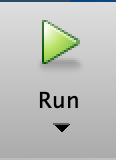
\includegraphics[width=0.52083in,height=\textheight]{run-button.png}}
de MATAB quand le script est sélectionné dans l'éditeur. On peut aussi
exécuter le script en appelant le nom du script dans la fenêtre de
commande sans son extension.

\hypertarget{commentaires}{%
\subsection{Commentaires}\label{commentaires}}

Les commentaires\footnote{\href{https://www.mathworks.com/help/matlab/matlab_prog/comments.html}{Add
  Comments to Programs}} sont des notes laissés par le programmeur qui
ne sera pas exécuté par MATLAB. Les commentaires permettent de laisser
des explications utiles sur les instructions dans nos programmes. Les
commentaires commencent avec un symbole de pourcentage
(\passthrough{\lstinline!\%!}) et le restant de la ligne est
automatiquement en commentaire. Une ligne suivant les points de
suspension terminant un commentaire est elle aussi considérée comme tel.

\hypertarget{arruxeat-durgence-dun-programme}{%
\subsection{Arrêt d'urgence d'un
programme}\label{arruxeat-durgence-dun-programme}}

Si MATLAB ne répond plus ou est constamment ``Busy'', on peut
interrompre\footnote{\href{https://www.mathworks.com/help/matlab/matlab_env/stop-execution.html}{Stop
  Execution}} le programme courant avec le raccourci
\passthrough{\lstinline!Ctrl-C!} après avoir sélectionné la fenêtre de
commande. Plusieurs annulations peuvent être nécessaires si plusieurs
opérations étaient en attente.

\hypertarget{fonctions-de-bases}{%
\section{Fonctions de bases}\label{fonctions-de-bases}}

Plusieurs fonctions simples sont utiles en commençant l'utilisation de
MATLAB.

\begin{itemize}
\tightlist
\item
  \passthrough{\lstinline!clc!}\footnote{\href{https://www.mathworks.com/help/matlab/ref/clc.html}{\passthrough{\lstinline!clc!}}}
  - Vide la fenêtre de commande
\item
  \passthrough{\lstinline!clear!}\footnote{\href{https://www.mathworks.com/help/matlab/ref/clear.html}{\passthrough{\lstinline!clear!}}}
  - Vide l'espace de travail
\item
  \passthrough{\lstinline!help!}\footnote{\href{https://www.mathworks.com/help/matlab/ref/help.html}{\passthrough{\lstinline!help!}}}
  fonction - Donne de l'aide sommaire sur la fonction
\item
  \passthrough{\lstinline!doc!}\footnote{\href{https://www.mathworks.com/help/matlab/ref/doc.html}{\passthrough{\lstinline!doc!}}}
  fonction - Donne la documentation sur la fonction
\end{itemize}

\hypertarget{variables}{%
\section{Variables}\label{variables}}

Une variable est l'unité de mémoire de base de nos programmes. Une
variable consiste en 3 choses :

\begin{itemize}
\tightlist
\item
  Un identificateur - Le nom de la variable
\item
  Une valeur - Le contenu de la variable
\item
  Un type - La nature de la variable
\end{itemize}

On crée une variable avec une instruction d'assignation. L'assignation
utilise le sigle égal (\passthrough{\lstinline!=!}) pour indiquer
l'assignation d'une expressions à un identificateur.\footnote{L'assignation
  se fait toujours d'une expression à droite vers un identificateur à
  gauche.} Pour utiliser une variable déjà assignée, on place son
identificateur à l'intérieur d'une expression. La valeur contenue dans
la variable sera remplacée dans l'expression avant qu'elle ne soit
évaluée.

\hypertarget{type-de-donnuxe9es}{%
\section{Type de données}\label{type-de-donnuxe9es}}

Les variables de MATLAB peuvent avoir plusieurs formes\footnote{\href{https://www.mathworks.com/help/matlab/matlab_prog/fundamental-matlab-classes.html}{Fundamental
  MATLAB Classes}}. Nous nous concentrerons sur trois types de variables
durant le début du cours.

\begin{itemize}
\tightlist
\item
  Valeurs numériques - \passthrough{\lstinline!double!}
\item
  Valeurs logiques - \passthrough{\lstinline!logical!}
\item
  Valeurs textuelles\footnote{Les valeurs textuelles sont appelées
    chaine de caractères.} - \passthrough{\lstinline!char!}
\end{itemize}

\hypertarget{double}{%
\subsection{\texorpdfstring{\texttt{double}}{double}}\label{double}}

Pour les variables numériques, le type
\passthrough{\lstinline!double!}\footnote{\href{https://www.mathworks.com/help/matlab/ref/double.html}{\passthrough{\lstinline!double!}}}
est utilisé par défaut dans MATLAB. Ce type est capable de contenir des
nombres réels de tout genre. Il existe une problématique avec le type
numérique double. Dû à la gestion de la mémoire pour représenter les
valeurs\footnote{\href{https://www.mathworks.com/help/matlab/matlab_prog/floating-point-numbers.html}{Floating-Point
  Numbers}}, il est souvent difficile de faire des comparaisons entre
deux valeurs qui sont supposées être identiques\footnote{Exemple :
  Essayez de faire \passthrough{\lstinline!0.3 - 0.2 - 0.1!} dans la
  fenêtre de commande.}. Pour faire des comparaisons de valeurs
calculées, on veut utiliser une comparaison entre une valeur minimale
(ex: 0.01) et la différence absolue des deux valeurs.

\hypertarget{logical}{%
\subsection{\texorpdfstring{\texttt{logical}}{logical}}\label{logical}}

Pour des éléments logiques binaires, le type
\passthrough{\lstinline!logical!}\footnote{\href{https://www.mathworks.com/help/matlab/ref/logical.html}{\passthrough{\lstinline!logical!}}}
est utilisé. Ce type peut avoir seulement deux possibilités:
\passthrough{\lstinline!true!}\footnote{\href{https://www.mathworks.com/help/matlab/ref/true.html}{\passthrough{\lstinline!true!}}}
ou \passthrough{\lstinline!false!}\footnote{\href{https://www.mathworks.com/help/matlab/ref/false.html}{\passthrough{\lstinline!false!}}},
représentées aussi par les valeurs 1 et 0 respectivement.

\hypertarget{char}{%
\subsection{\texorpdfstring{\texttt{char}}{char}}\label{char}}

Pour sauvegarder du texte, le type
\passthrough{\lstinline!char!}\footnote{\href{https://www.mathworks.com/help/matlab/ref/char.html}{\passthrough{\lstinline!char!}}}
est disponible. Les variables sont capables de contenir des chaines de
caractères.\footnote{Des chaines de caractères sont nommées
  ``\passthrough{\lstinline!string!}'' en anglais. Il faut faire
  attention par contre, car il existe un type
  \passthrough{\lstinline!string!} dans MATLAB, mais celui-ci ne sera
  pas utilisé dans le cours, nous utiliserons des ``character vectors''
  de type \passthrough{\lstinline!char!}.} Les chaines des caractères
sont représentées par du texte à l'intérieur de guillemets simples.

\hypertarget{constantes}{%
\subsection{Constantes}\label{constantes}}

Durant la création de nos programmes, il nous est donné d'utiliser des
valeurs arbitraires pour représenter des informations (taux de taxation,
âge minimum, etc.) Pour augmenter la lisibilité du code et éviter des
erreurs, ce genre de valeurs doit être contenu dans des variables avec
des identificateurs spéciaux. Les constantes auront des noms de
variables constitués seulement de lettres en majuscules pour les
différences des variables typiques. Si notre programme à besoin de
plusieurs variables, il est habituel de les regrouper dans un script et
d'appeler le script au moment opportun.

\hypertarget{fprintf}{%
\section{\texorpdfstring{\texttt{fprintf}}{fprintf}}\label{fprintf}}

La fonction \passthrough{\lstinline!fprintf!}\footnote{\href{https://www.mathworks.com/help/matlab/ref/fprintf.html}{\passthrough{\lstinline!fprintf!}}}
permet d'afficher de l'information dans la fenêtre de commande. Son
utilisation de base est simple, mais elle contient plusieurs
configurations optionnelles. La version la plus simple du
\passthrough{\lstinline!fprintf!} affiche le contenu d'une chaine de
caractères envoyé en paramètre.

\begin{lstlisting}[language=Matlab]
fprintf('Bonjour la vie!\n')
fprintf('Bonjour la vie!\n')
fprintf('Bonjour la vie!\n')
\end{lstlisting}

\end{document}
